% SIAM Shared Information Template
% This is information that is shared between the main document and any
% supplement. If no supplement is required, then this information can
% be included directly in the main document.

In this section we study the impact of parameter $\epsilon_s$ and hardware parallelism on the quality of  RACE method. \Inorder to do this we first quantify the quality of the method and finally we  use this quantity to do a parameter study. The study gives insights into tuning of parameter $\epsilon_s$ based on the given matrix and required parallelism.


\subsection{Quantifying quality of RACE}
Quantifying quality of the method in a well-defined way is a primary and most vital step for parameter study. We do this using the concept of \effPar. From \cref{Sec:race} we saw that even though one tries to achieve parallelism exactly as that required by the hardware, in practice one might not be able to utilize this parallelism to 100 \% due to load imbalances. Therefore we use a simple calculation based on the \levelTree to determine efficiency. This takes into account load imbalances incurred from different stages of recursion. We first calculate \effRow for each of the worker leaves (leaves in finest level) in \levelTree.
The \levelGroups (leaves) in \levelTree that are not further refined form worker leaves and they are responsible for executing the rows (nodes) in their range, the work done by these leaves is therefore directly proportional to the number of rows. Hence the \effRow of these worker leaves is same as number of rows (\nrows), for example in case of $T_0(0)$ \effRow ( $\nrowsEffMath(T_0(0))$ = $\nrowsMath(T_0(0))$ ) is 14 and $\nrowsEffMath(T_1(0) \subset T_0(4))$ is 6. After calculating the \effRow for worker leaves the information is propagated to other leaves in lower stages (up in the \levelTree) as follows: 
\begin{align*}
\nrowsEffMath(T_s(i)) &= max(\nrowsEffMath(T_{s+1}(j) \subset T_s(i))) + max(\nrowsEffMath(T_{s+1}(k) \subset T_s(i)))\\
 & \text{for } j \text{ is even and } k \text{ is odd}
\end{align*}

Such a definition for \effRow is based on the idea that a parent has to wait until the child leaf with most number of rows in each sweep (color) has finished it's work due to synchronization needed with it's siblings. This has to be handled separately for each of the two parallel sweep (colors) as there is this synchronization happening after each of the sweeps (colors). 

Once the information is propagated up the tree and as it reaches the root we have a single \effRow ($\nrowsEffMath(T_{-1})$) for the entire tree, which has taken into account load imbalance happening between all \levelGroups in all stages. The ratio of total number of rows ($\nrowsMath^{total}$) in the entire matrix to that of $\nrowsEffMath(T_{-1})$ gives \effPar, denoted as \threadEff. Efficiency ($\eta$) of the method is then defined as ratio of  \threadEff to that of required hardware parallelism (\nthreads). 

\begin{align}
	\threadEffMath &= \frac{\nrowsMath^{total}}{\nrowsEffMath(T_{-1})} \\
	\eta &= \frac{\threadEffMath}{\nthreadsMath} \label{eq:eta}
\end{align}

For example in our \stex, \cref{fig:rec_2d-7pt_tree} shows \nrowsEff for each leaves in angular brackets and here $\threadEffMath = 5.8$ and $\eta = 0.725$. The value of $\eta = 1$ implies there is perfect load balancing which is almost impossible. In general $0 < \eta \leq 1$. This parameter $\eta$ will be used as a measure of quality in parameter study.

\subsection{Case study}
A given matrix has a fixed amount of parallelism and as the amount of required parallelism (\nthreads) increases load balancing degrades due to more threads per stage and imbalances between stages. The rate of degradation can however be controlled to certain extent by the tolerance $\epsilon_s$ (see \cref{eq:epsilon}) specified while choosing a \levelGroup. Typical value of $\epsilon_s$ is in range of [0.4,0.9]. Having a small $\epsilon_s$ (for example 0.4) implies we utilize the current stage `s' to maximum and do not impose high load balancing constraint, a high value on the other hand requires more balanced load from current stage `s'. 

Test matrices (see \cref{Sec:test_bed}) considered have a varying degree of parallelism, and in order to see the effect of $\eta$ and $\epsilon_s$ we choose the \emph{inline} matrix. The choice is due to the fact that this matrix has relatively small amount of parallelism and this allows us to demonstrate various effect, ranging from good to bad case scenario with small number of parallelism (\nthreads$ < 200$). This limited parallelism can be observed from \cref{fig:inline-a} 
where efficiency keeps on decreasing with \nthreads for \emph{inline} matrix. Similar behavior can be observed for \emph{crankseg\_1}, \emph{F1} and \emph{ship} matrices, of which \emph{crankseg\_1} being the worst. For majority of other test matrices one could observe that efficiency $\eta$ initially drops but then remains almost constant in the range $\eta$ = [0.50,0.80] (depending on matrix) for the entire scanned area of $1 \leq $\nthreads$ \leq 200$.

\begin{figure}[tbhp]
	\centering
	\subfloat[$\eta$ vs \nthreads for \emph{inline} matrix ]{\label{fig:inline-a}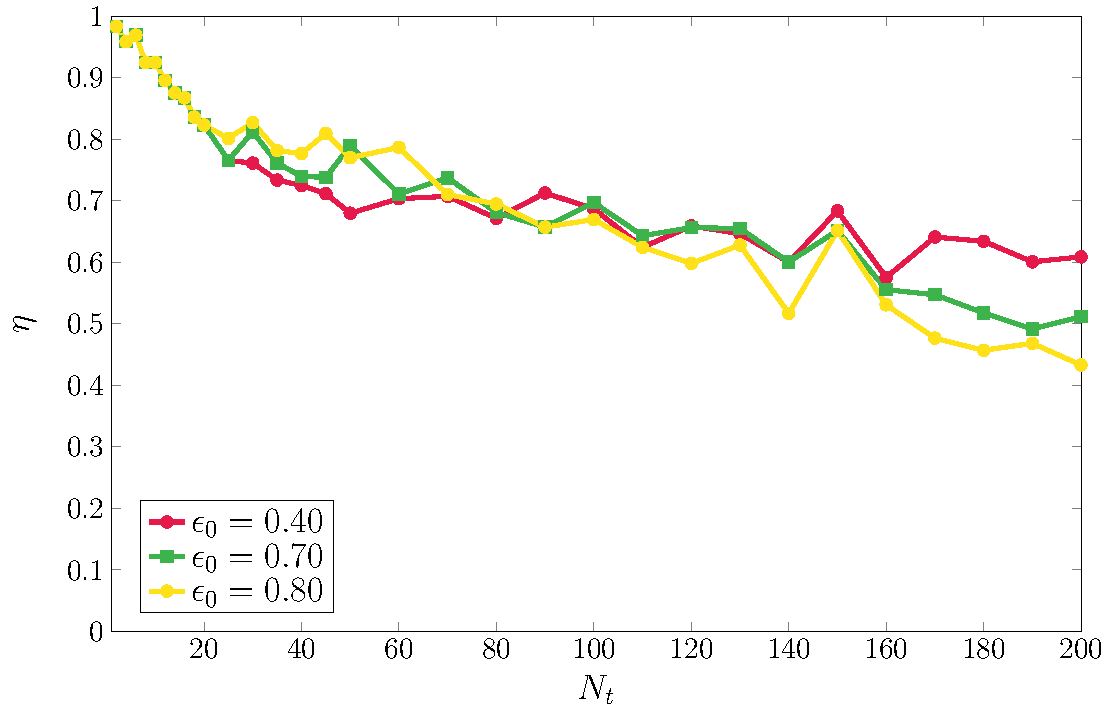
\includegraphics[width=0.45\textwidth , height=0.2\textheight]{pics/param_study/threads_vs_eff}}
	\hspace{1.5em}
	\subfloat[Effect of $\epsilon_1$ at low \nthreads, \nthreads=25]{\label{fig:inline-b}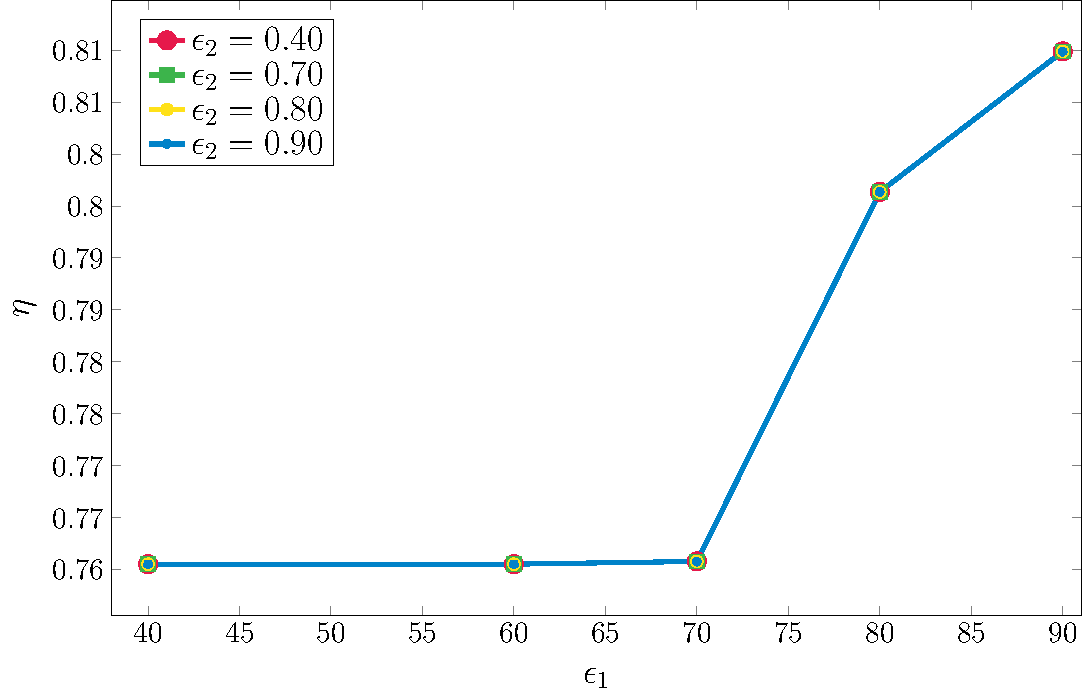
\includegraphics[width=0.45\textwidth , height=0.2\textheight]{pics/param_study/scaling_eps_1_25_threads}}
	
	\subfloat[Optimal $\epsilon_1$ lowered and optimal $\epsilon_2$ = 0.9, \nthreads=45 ]{\label{fig:inline-c}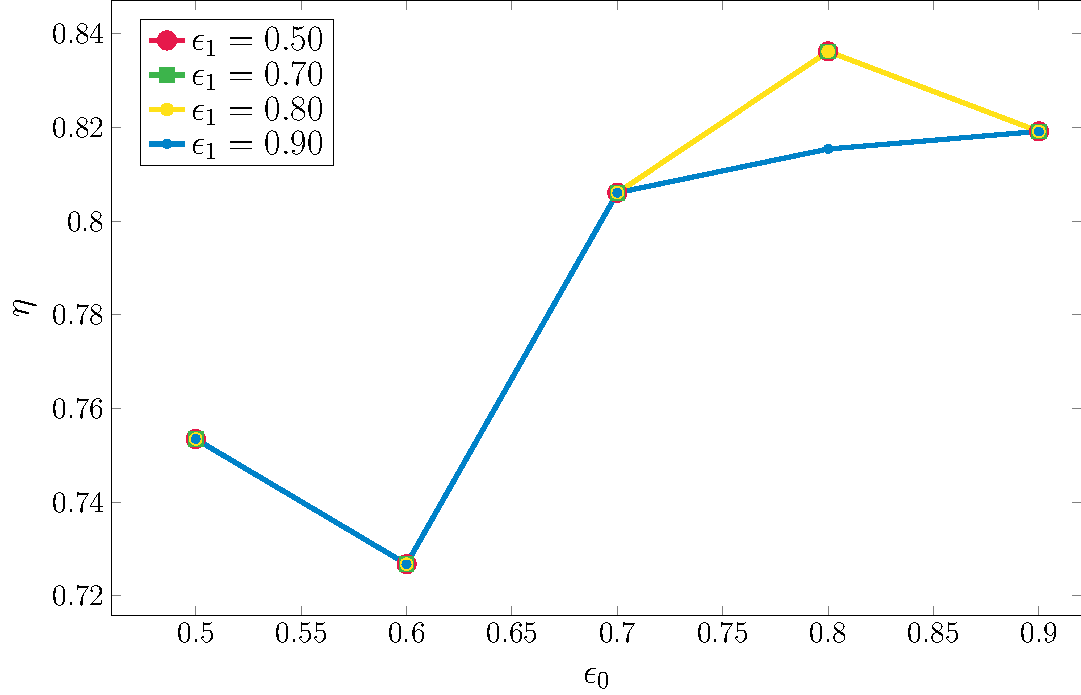
\includegraphics[width=0.45\textwidth , height=0.2\textheight]{pics/param_study/scaling_eps_1_45_threads}}
	\hspace{1.5em}
	\subfloat[Optimal $\epsilon_1$ lowered to 0.4 and $\epsilon_2$ to 0.7, \nthreads=190 ]{\label{fig:inline-d}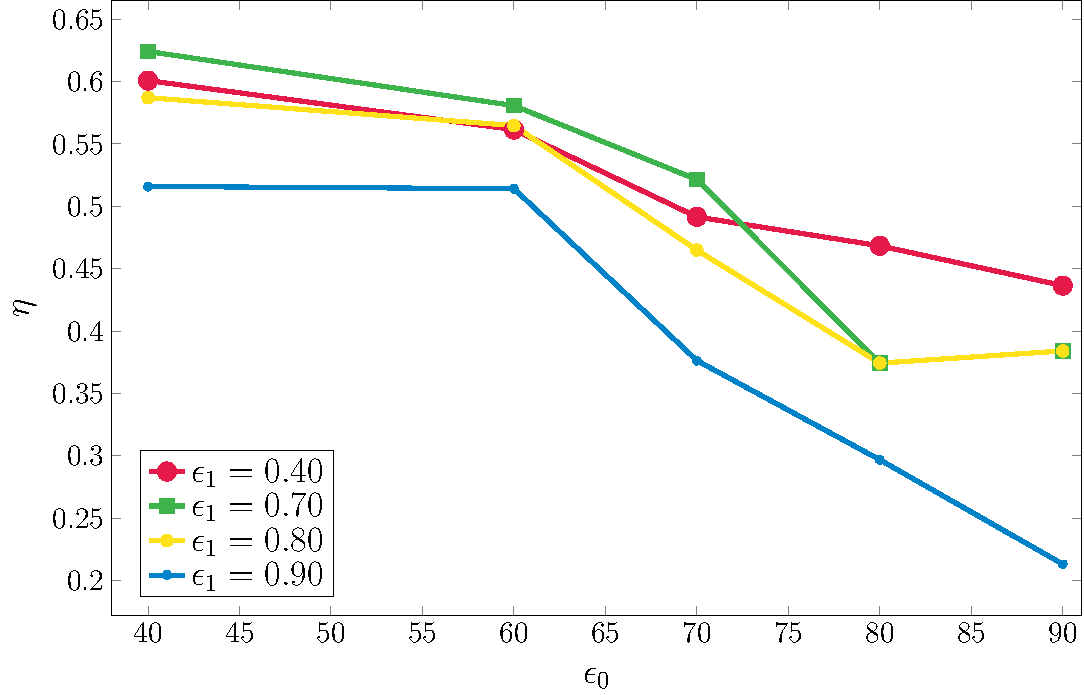
\includegraphics[width=0.45\textwidth , height=0.2\textheight]{pics/param_study/scaling_eps_1_190_threads}}
	\caption{Parameter study on \emph{inline} matrix. In \cref{fig:inline-b,fig:inline-c,fig:inline-d} each lines in the plot are iso-$\epsilon_2$ and impact of $\eta$ with respect to $\epsilon_1$ is shown.}
	\label{fig:inline_param_study}
\end{figure}

At small number of threads (\nthreads) all matrices have high efficiency (like $\eta>0.8$). As there is a lot of parallelism in this stage compared to requirement, $\eta$ is insensitive of $\epsilon_s$. The value of \nthreads upto which such a behavior can be observed varies from matrix to matrix, for example \emph{inline} shows this upto \nthreads$\approx20$, while for matrix like \emph{Graphene} this is grater than $200$.  Further increasing \nthreads one could observe $\eta$ starts to vary with $\epsilon_0$. For example in case of \nthreads$ = 25$ one could see in \cref{fig:inline-b} maximum $\eta$ is achieved with high value of $\epsilon_0$ (0.9) due to good load balancing. But as 
\nthreads further increase the optimal $\epsilon_0$ starts shifting towards left (see \cref{fig:inline-c}),
 since one requires more parallelism from the current stage (s=0) and higher $\epsilon_0$ would be decremental since it would require the \levelTree to go more deep and hence load imbalances in next stages will get multiplied. $\epsilon_1$ which till now didn't effect much starts to influence slowly as \nthreads increments again, for example in case of \emph{inline} till $\nthreadsMath=90$ $\epsilon_1=0.9$ was optimal, but then the optimal $\epsilon_1$ reduces and reaches $0.7$ at \nthreads$=190$ as seen in \cref{fig:inline-d}. $\eta$ would start to get affected by $\epsilon_s$ of next stages in similar manner with increase of \nthreads.
 
   \begin{figure}[tbhp]
   	\centering
   	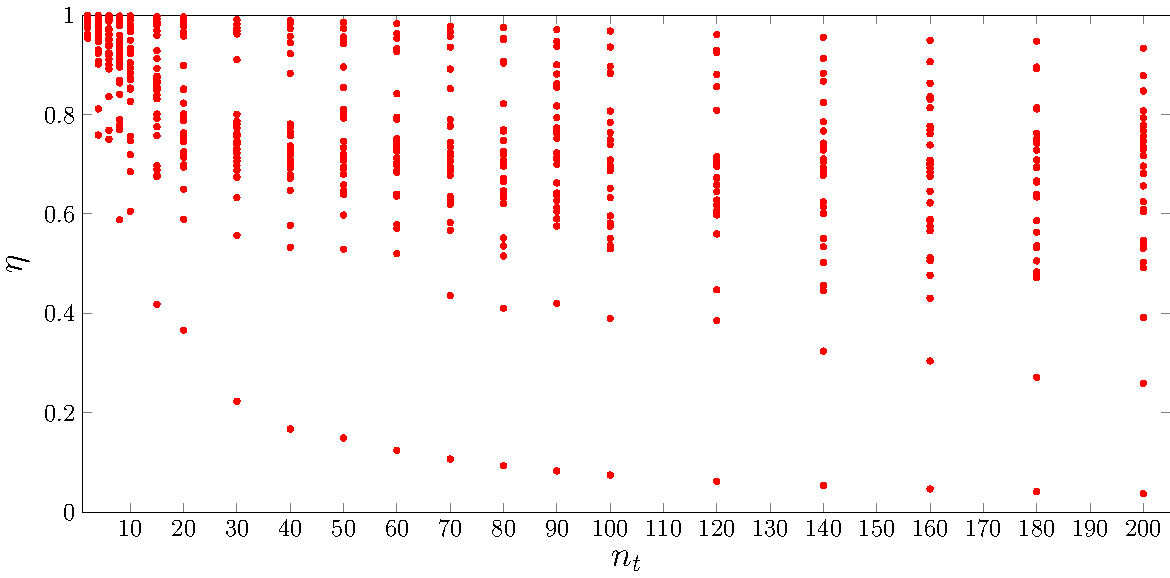
\includegraphics[height=0.18\textheight,width=\textwidth]{pics/param_study/scatter_plot}
   	\caption{Scatter plot of $\eta$ vs \nthreads of all test matrices, with $\epsilon_s$ = 0.4}
   	\label{fig:param_all_mtx_stat}
   \end{figure}
   
Behavior of other matrices in the test bed follow similar pattern, but \nthreads at which different phases occur varies from matrix to matrix.  \Cref{fig:param_all_mtx_stat} gives a broad overview of the efficiency ($\eta$) behavior of entire test matrices using scatter plot. Each point at a specific \nthreads represents efficiency ($\eta$) of a matrix. Majority of test matrices having an initial drop in $\eta$ and then remaining constant is reflected in the statistical plot. The lowest points in the plot correspond to \emph{crankseg\_1} matrix, here we achieve only a mere parallelism of eight at maximum (\threadEff = 8), while the upper points correspond to matrix having highest parallelism namely \emph{Graphene} matrix.

In practice for a given matrix it's difficult to precisely determine the optimal rate of decrease in $\epsilon_s$ without parameter search, and therefore selecting proper $\epsilon_s$ for given \nthreads can be challenging. One idea is to see total levels (\totalLvl) and distribution of non-zeros (\nnz) in different levels of current stage `s' and heuristically determine $\epsilon_s$ based on the pressure of parallelism from stage `s'. This is not currently done and is part of our future work. As a rule of thump an $\epsilon_{0,1} = 0.8$ and $\epsilon_{s>1} = 0.4$ is sufficient for most matrices on current architectures, therefore currently for experiments we set these $\epsilon_s$ values for all matrices.

\begin{figure}[tbhp]
	\centering
	\subfloat[\emph{crankseg\_1}]{\label{fig:crankseg_param}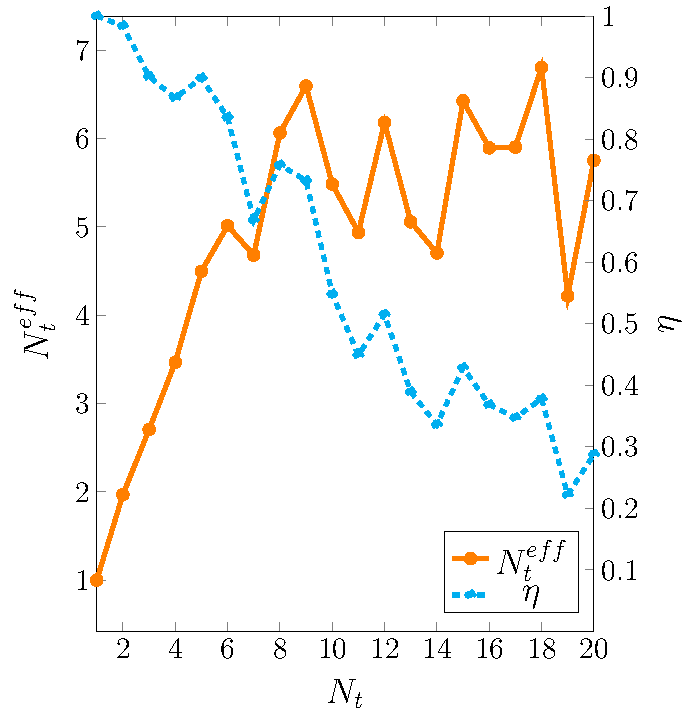
\includegraphics[width=0.23\textwidth , height=0.16\textheight]{pics/param_study/corner_cases/crankseg_1}}
	\subfloat[\emph{inline\_1}]{\label{fig:inline_param}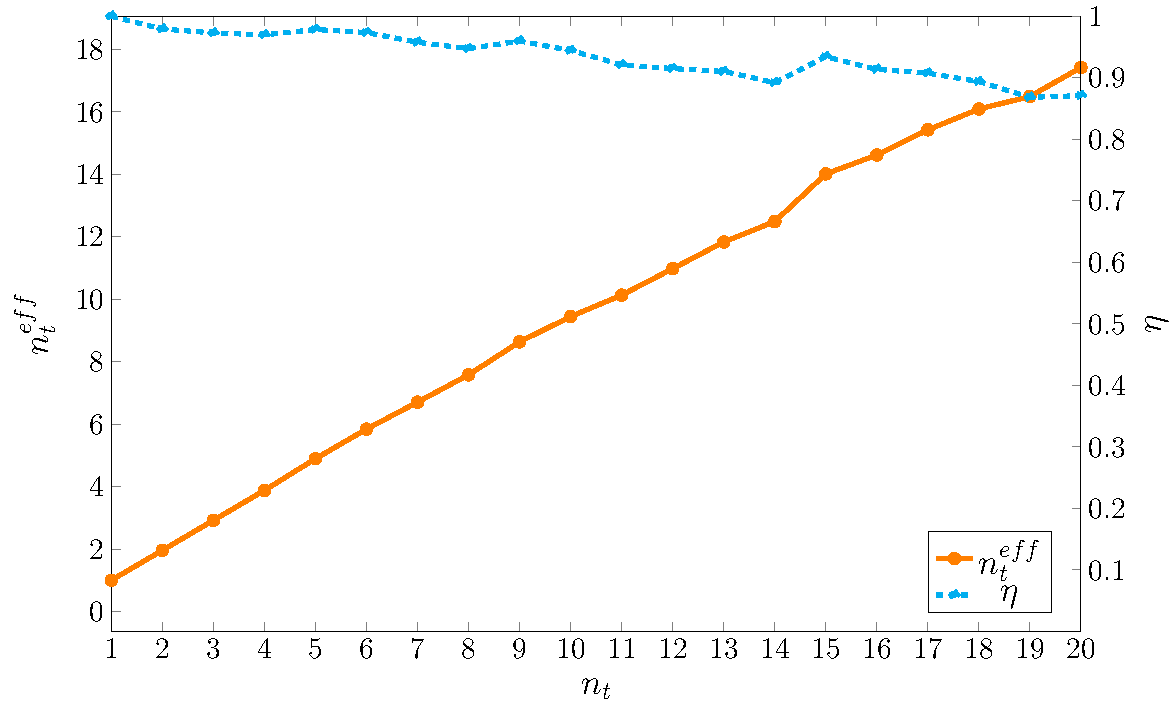
\includegraphics[width=0.23\textwidth , height=0.16\textheight]{pics/param_study/corner_cases/inline_1}}	
	\subfloat[\emph{parabolic\_fem}]{\label{fig:parabolic_fem_param}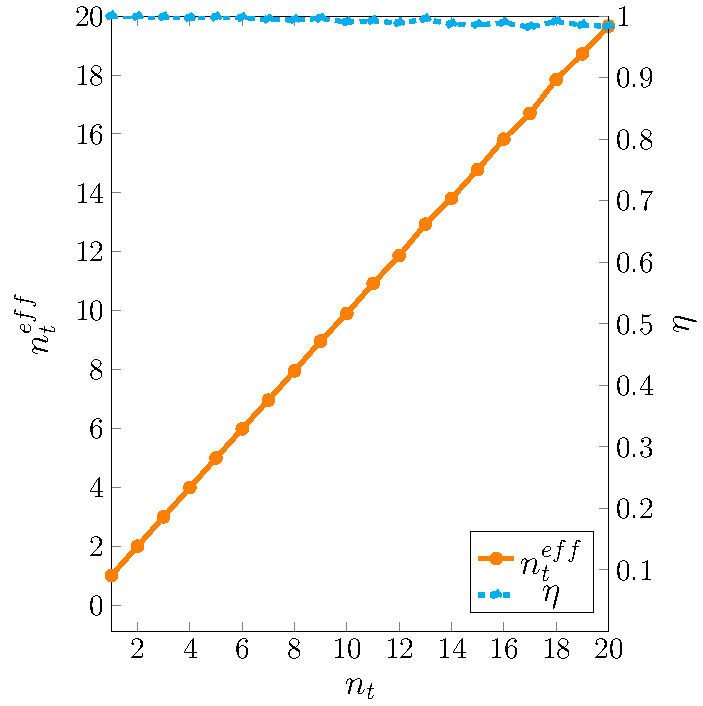
\includegraphics[width=0.23\textwidth , height=0.16\textheight]{pics/param_study/corner_cases/parabolic_fem}}
	\subfloat[\emph{Graphene-4096}]{\label{fig:Graphene-4096_param}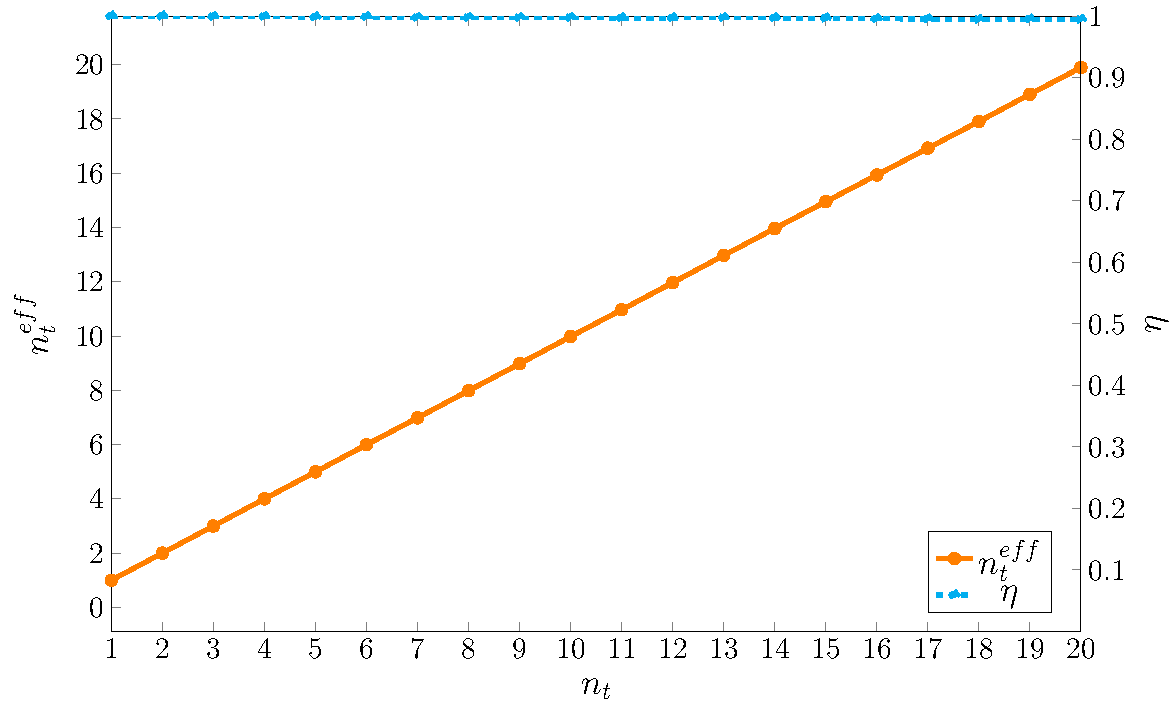
\includegraphics[width=0.23\textwidth , height=0.16\textheight]{pics/param_study/corner_cases/Graphene-4096}}	
	\caption{\threadEff and $\eta$ vs \nthreads for corner case matrices, with the same settings used in experiment runs. \threadEff is defined as $\eta$ * \nthreads.}
	\label{fig:corner_cases_param}
\end{figure}
\begin{figure}[tbhp]
	\centering
	\subfloat[\emph{crankseg\_1}]{\label{fig:crankseg_scaling}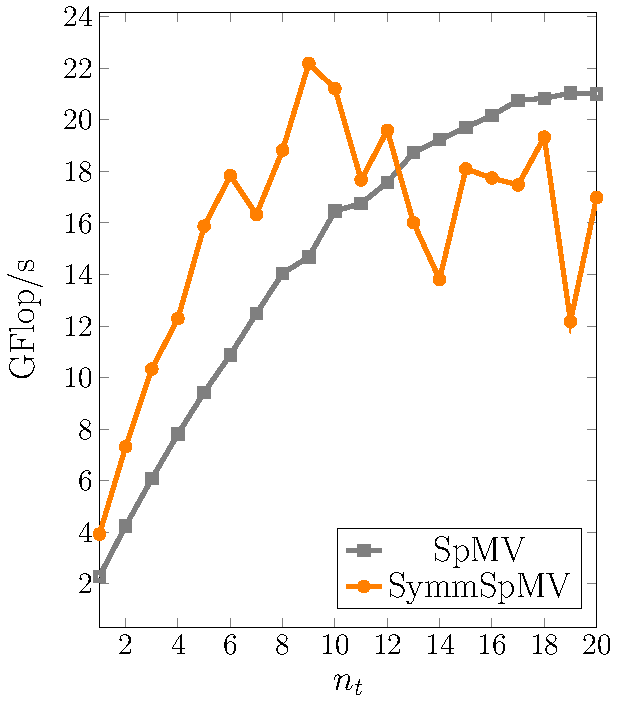
\includegraphics[width=0.23\textwidth , height=0.18\textheight]{pics/results/skx/corner_cases_scaling/plots/RCM/crankseg_1}}
	\subfloat[\emph{inline\_1}]{\label{fig:inline_scaling}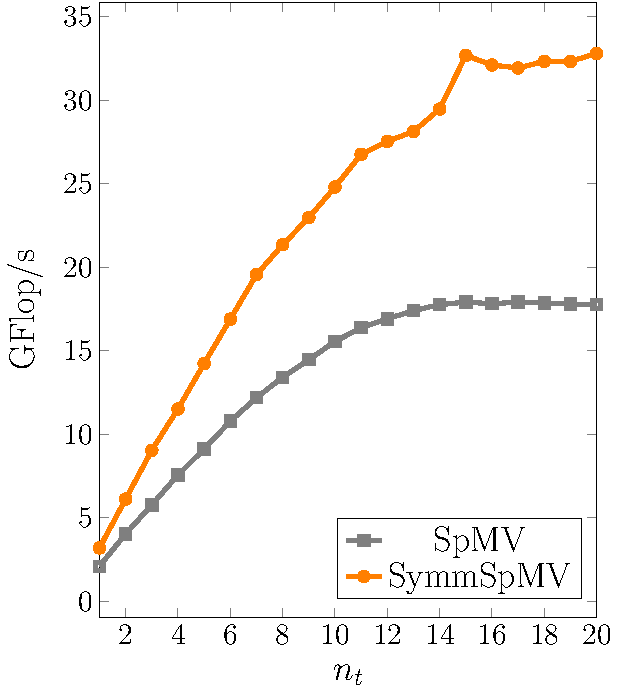
\includegraphics[width=0.23\textwidth , height=0.18\textheight]{pics/results/skx/corner_cases_scaling/plots/RCM/inline_1}}	
	\subfloat[\emph{parabolic\_fem}]{\label{fig:parabolic_fem_scaling}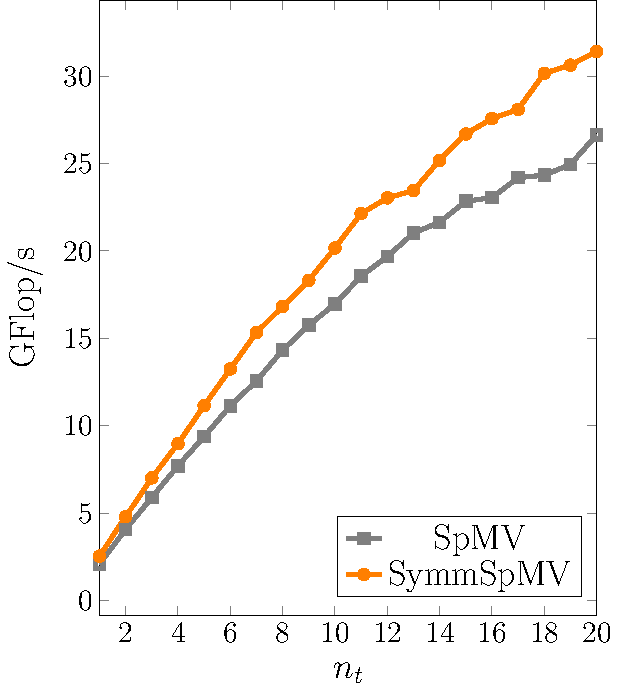
\includegraphics[width=0.23\textwidth , height=0.18\textheight]{pics/results/skx/corner_cases_scaling/plots/RCM/parabolic_fem}}
	\subfloat[\emph{Graphene-4096}]{\label{fig:Graphene-4096_scaling} 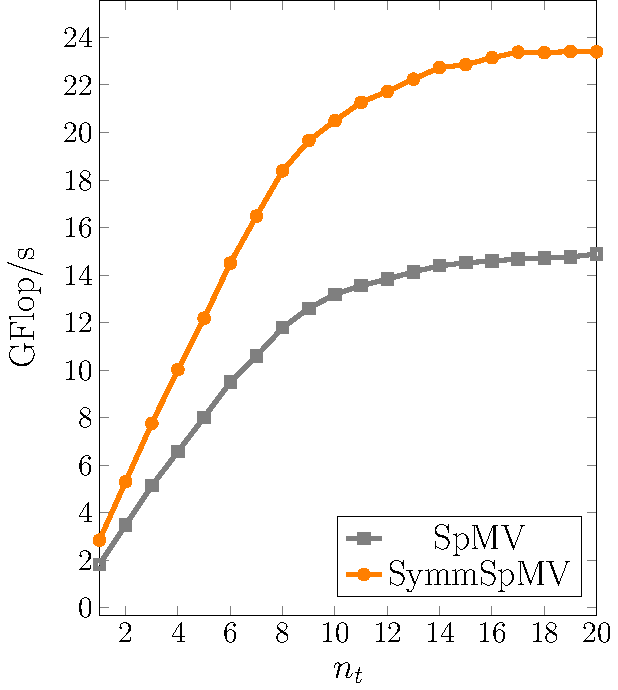
\includegraphics[width=0.23\textwidth , height=0.18\textheight]{pics/results/skx/corner_cases_scaling/plots/RCM/Graphene-4096}}	
	\caption{Scaling of \SymmSpmv with RACE compared to \SpMV on one socket of \SKX architecture, for corner case matrices.}
	\label{fig:corner_cases_scaling}
\end{figure}
 In \cref{fig:corner_cases_param} we have plotted \threadEff and $\eta$ vs \nthreads for corner case matrices with the settings used in experiment runs. Here we set $\epsilon_{0,1}=0.8$ and use \RCM (\RCMfull) in the \emph{level construction} stage (\cref{subsec:LEVEL_CONST}). Big fluctuation in \emph{crankseg\_1} is due to the fact that we set high load balancing requirement (high $\epsilon_s$ factor) and as seen in the example of \emph{inline\_1} matrix this is not optimal when we reach the limit of parallelism. The theoretical estimates obtained in \cref{fig:corner_cases_param} will be directly used to compare with experiment runs in the next section (\cref{Sec:expt}).

